% AEJ-Article.tex for AEA last revised 22 June 2011
\documentclass[AEJ]{AEA}

%%%%%% NOTE FROM OVERLEAF: The mathtime package is no longer publicly available nor distributed. We recommend using a different font package e.g. mathptmx if you'd like to use a Times font.
%\usepackage{mathptmx}
\usepackage{graphicx}
\usepackage{subcaption}
\usepackage{float}
\usepackage{longtable,booktabs,array}

% The mathtime package uses a Times font instead of Computer Modern.
% Uncomment the line below if you wish to use the mathtime package:
%\usepackage[cmbold]{mathtime}
% Note that miktex, by default, configures the mathtime package to use commercial fonts
% which you may not have. If you would like to use mathtime but you are seeing error
% messages about missing fonts (mtex.pfb, mtsy.pfb, or rmtmi.pfb) then please see
% the technical support document at http://www.aeaweb.org/templates/technical_support.pdf
% for instructions on fixing this problem.

% Note: you may use either harvard or natbib (but not both) to provide a wider
% variety of citation commands than latex supports natively. See below.

% Uncomment the next line to use the natbib package with bibtex 
\usepackage{natbib}

% Uncomment the next line to use the harvard package with bibtex
%\usepackage[abbr]{harvard}

% This command determines the leading (vertical space between lines) in draft mode
% with 1.5 corresponding to "double" spacing.
\draftSpacing{1.5}

\begin{document}

\title{The Impact of the Odd-Even Policy in Jakarta on Road Pollution}
\shortTitle{}
\author{Ardhi Wardhana, Faiz Phillarete and Rio Pramudita\thanks{%
Wardhana: Columbia University, 420 W 118th St, New York, NY 10027, arw2222@columbia.edu. Philarette: Columbia University, 420 W 118th St, New York, NY 10027, fep2119@columbia.edu, Pramudita: Columbia University, 420 W 118th St, New York, NY 10027, rpk2133@columbia.edu. Thanks to Dr. Harold Stolper and the teaching team for conducting a great course}}
\date{\today}
\pubMonth{}
\pubYear{}
\pubVolume{}
\pubIssue{}
\JEL{}
\Keywords{}

\begin{abstract}
This study examines the impact of the odd-even policy on reducing pollutant emissions in Jakarta. By using an event study - two-way fixed-effect, this study found a reduction in PM 2.5 on roads that implemented the policy in Jakarta, albeit at a relatively modest scale. The study identifies potential loopholes in policy efficacy, such as user shifts to motorcycles or acquiring additional vehicles with different plate numbers. Despite these challenges, the study advocates for the expansion of the policy, citing the limited alternatives available to address air pollution DKI Jakarta. The findings underscore the importance of a comprehensive approach, taking into consideration enforcement mechanisms and user behaviors, to enhance the overall effectiveness of vehicle operation restrictions in mitigating air pollution.
\end{abstract}

\maketitle

In recent years, the air quality problem has become a persistent problem in Jakarta. The air quality of the Indonesian capital has deteriorated, with the Particulate Matter (PM) 2.5 average concentration escalating to 49.4 $\mu$g$/m^3$ in 2019, which is about 66\% higher than in 2017 (Zulkarnain et al, 2021). The deteriorating air quality imposes other problems on the nation's capital, as air pollution has been strongly linked to non-communicable diseases (NCDs), including cardiovascular and chronic respiratory diseases and lung cancers, which impose substantial burdens on the healthcare sector and the economy of the country (Syuhada et al, 2023). 

In 2019, Jakarta witnessed NCDs comprising 79\% (equivalent to 36,000 deaths) of the overall mortality rate. The impact of air pollution in generating NCDs and premature fatalities extends to significant consequences, including the loss of productive labor, escalated healthcare expenses, a decline in the country's gross domestic product (GDP), decreased productivity and competitiveness of cities, and a deterioration in the overall quality of life for residents. Recent findings from the World Bank revealed that the annual cost of air pollution in Indonesia exceeded USD 220 billion in 2019, constituting 6.6\% of the country's GDP (PPP).

Internal combustion engine (ICE) vehicles have become the primary source of pollution in Jakarta. In particular, the contribution of ICE vehicles to the PM2.5 concentration of Jakarta is approximately 32--57\%. This is due to the rapid motorization of Jakarta and its surrounding regions (Zulkarnain et al., 2021). The rapid motorization in Jakarta itself is a problem that has existed for a long time, with the average annual growth rate of motorized vehicles reaching 9.5 percent in 2017. 

In 1994, the government introduced the 3-in-1 policy in an attempt to manage the congestion on many main roads in  Jakarta. However, one of the latest policies to be introduced is the odd-even driving restrictions, a traffic management system enacted to curtail the travel of passenger cars on certain roads based on the vehicle license number. The odd-even policy was initially implemented during the 2018 Asian Games and only covered a small share of the main roads in Jakarta. Due to its perceived effect, it was expanded by the end of the event as a permanent policy that covered the 9 main roads in  Jakarta.

Some studies said the policy effectively reduces vehicles' travel time. However, the impact of the regulation on air quality remains in question, considering that many factors affect air quality. This brought up the policy question of this paper: How does Jakarta's odd-even traffic regulation policy affect air quality?

Several research studies have suggested that implementing transportation demand management (TDM) through restrictions on vehicle operations has reduced pollutant emissions by over 50\% (Bigazzi and Rouleau, 2017). New Delhi, for example, has already implemented the policy in 2016. In collaboration with Evidence for Policy Design, the Energy Policy Institute at the University of Chicago analyzed the effects of the odd-even scheme implemented in 2016. The study revealed that during the hours when the scheme was enforced in January of that year, Delhi experienced a 14-16\% decrease in PM2.5 levels. However, when the scheme was reintroduced in April of the same year, there was no discernible reduction in pollution. Similarly, this paper aims to analyze to what extent the odd-even policy could affect air quality, which will also be measured in PM2.5 levels.

\section{Policy Background}
The odd-even policy observed in this paper is the one that was applied after the Asian Games in Jakarta in September 2018. That policy was imposed on nine Jakarta primary roads from 6 AM to 9 PM every weekday. This policy was expanded in September 2019, adding 16 more streets being covered, thus bringing in 25 streets covered by the policy. This policy refers to the  Jakarta Governor's Regulation 155/2018 and the  Jakarta Governor's Regulation 88/2019. This study observed the change in these 2 time points, thus observing the monthly road data from April 2018 until March 2020.

This study used the roads where the odd-even policy was implemented as a treatment group in our paper to observe the effect of the policy on our pollution. In choosing our control group, this study looked for roads similar to the treated group's streets. Due to the limited availability of data on traffic and exact origin-destination data, this study used Jakarta's bus rapid transit (BRT) system route as our proxy. Jakarta's BRT amounted to 15 million monthly passengers, with coverage of 85\% of Jakarta, serving as one of the most extensive commuting services in  Jakarta. One of the features of the BRT is the route is parallel with the most crowded roads in Jakarta, therefore serving as a direct transportation alternative to private vehicles. 

This study overlayed the overlapping BRT routes with the main roads in Jakarta, and the initial visualization showed that it aligns with the roads that implement the odd-even policy. Therefore, this study used the roads that overlap with the BRT route as the controlled roads in this research.


\begin{figure}
    \centering

    \begin{subfigure}{0.3\textwidth}
        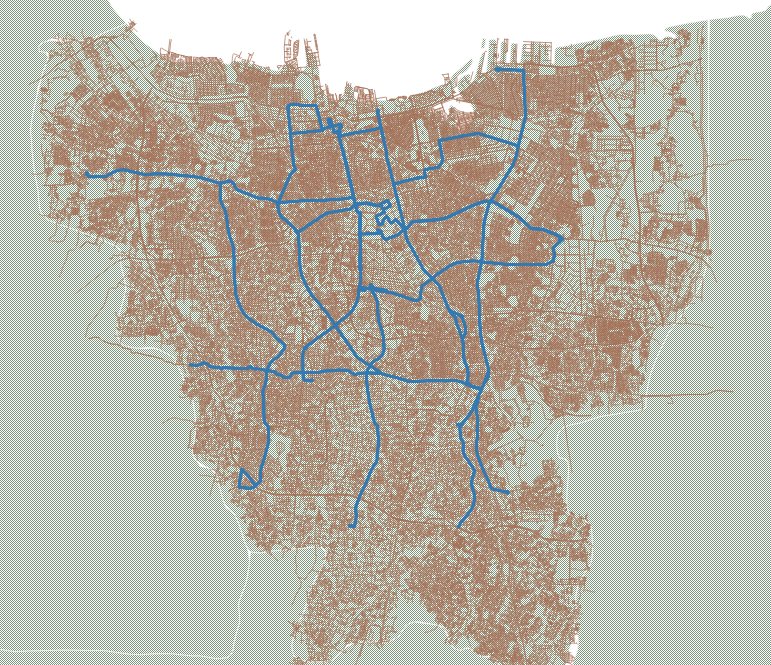
\includegraphics[width=1\linewidth]{Graphs/control.png}
        \caption{Control Group}
        \label{fig:sub1}
    \end{subfigure}
    \hfill
    \begin{subfigure}{0.3\textwidth}
        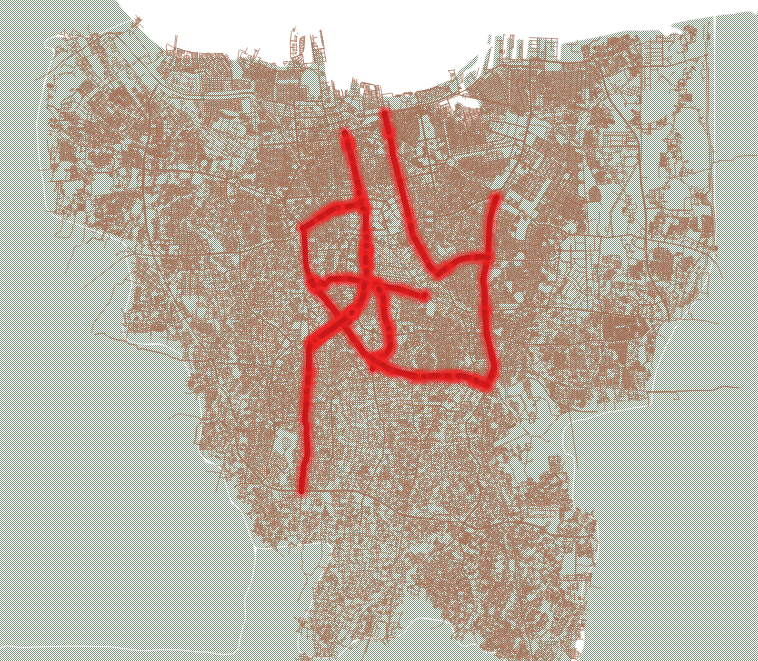
\includegraphics[width=1\linewidth]{Graphs/gage.png}
        \caption{Treated Group}
        \label{fig:sub2}
    \end{subfigure}
    \hfill
    \begin{subfigure}{0.3\textwidth}
        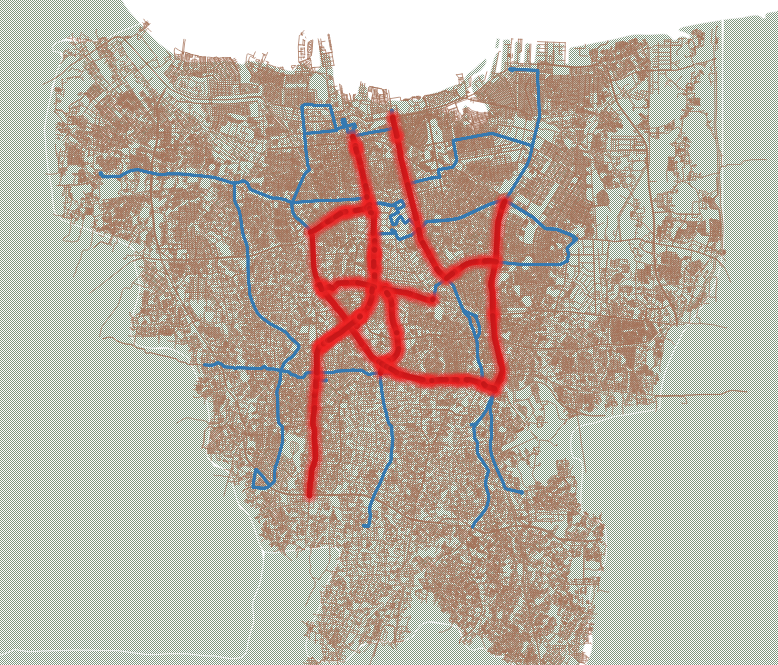
\includegraphics[width=1\linewidth]{Graphs/overlay.png}
        \caption{Overlaid Map}
        \label{fig:sub3}
    \end{subfigure}

    \caption{Control and Treatment Roads Group}
    \label{fig:overall}
\begin{figurenotes}
The control group is the roads that have never been enforced to apply the Odd-even policy. The treated group is the roads that applied the policy in September 2018 or August 2019.
\end{figurenotes}
\begin{figurenotes}[Source]
Author's visualization using ArcGIS.
\end{figurenotes}
\end{figure}

\vspace{-2.2em}
\section{Data}
\vspace{-1em}
\subsection{Particulate Matter 2.5}
\vspace{-0.5em}

\begin{figure}
    \hspace*{0.5cm}
    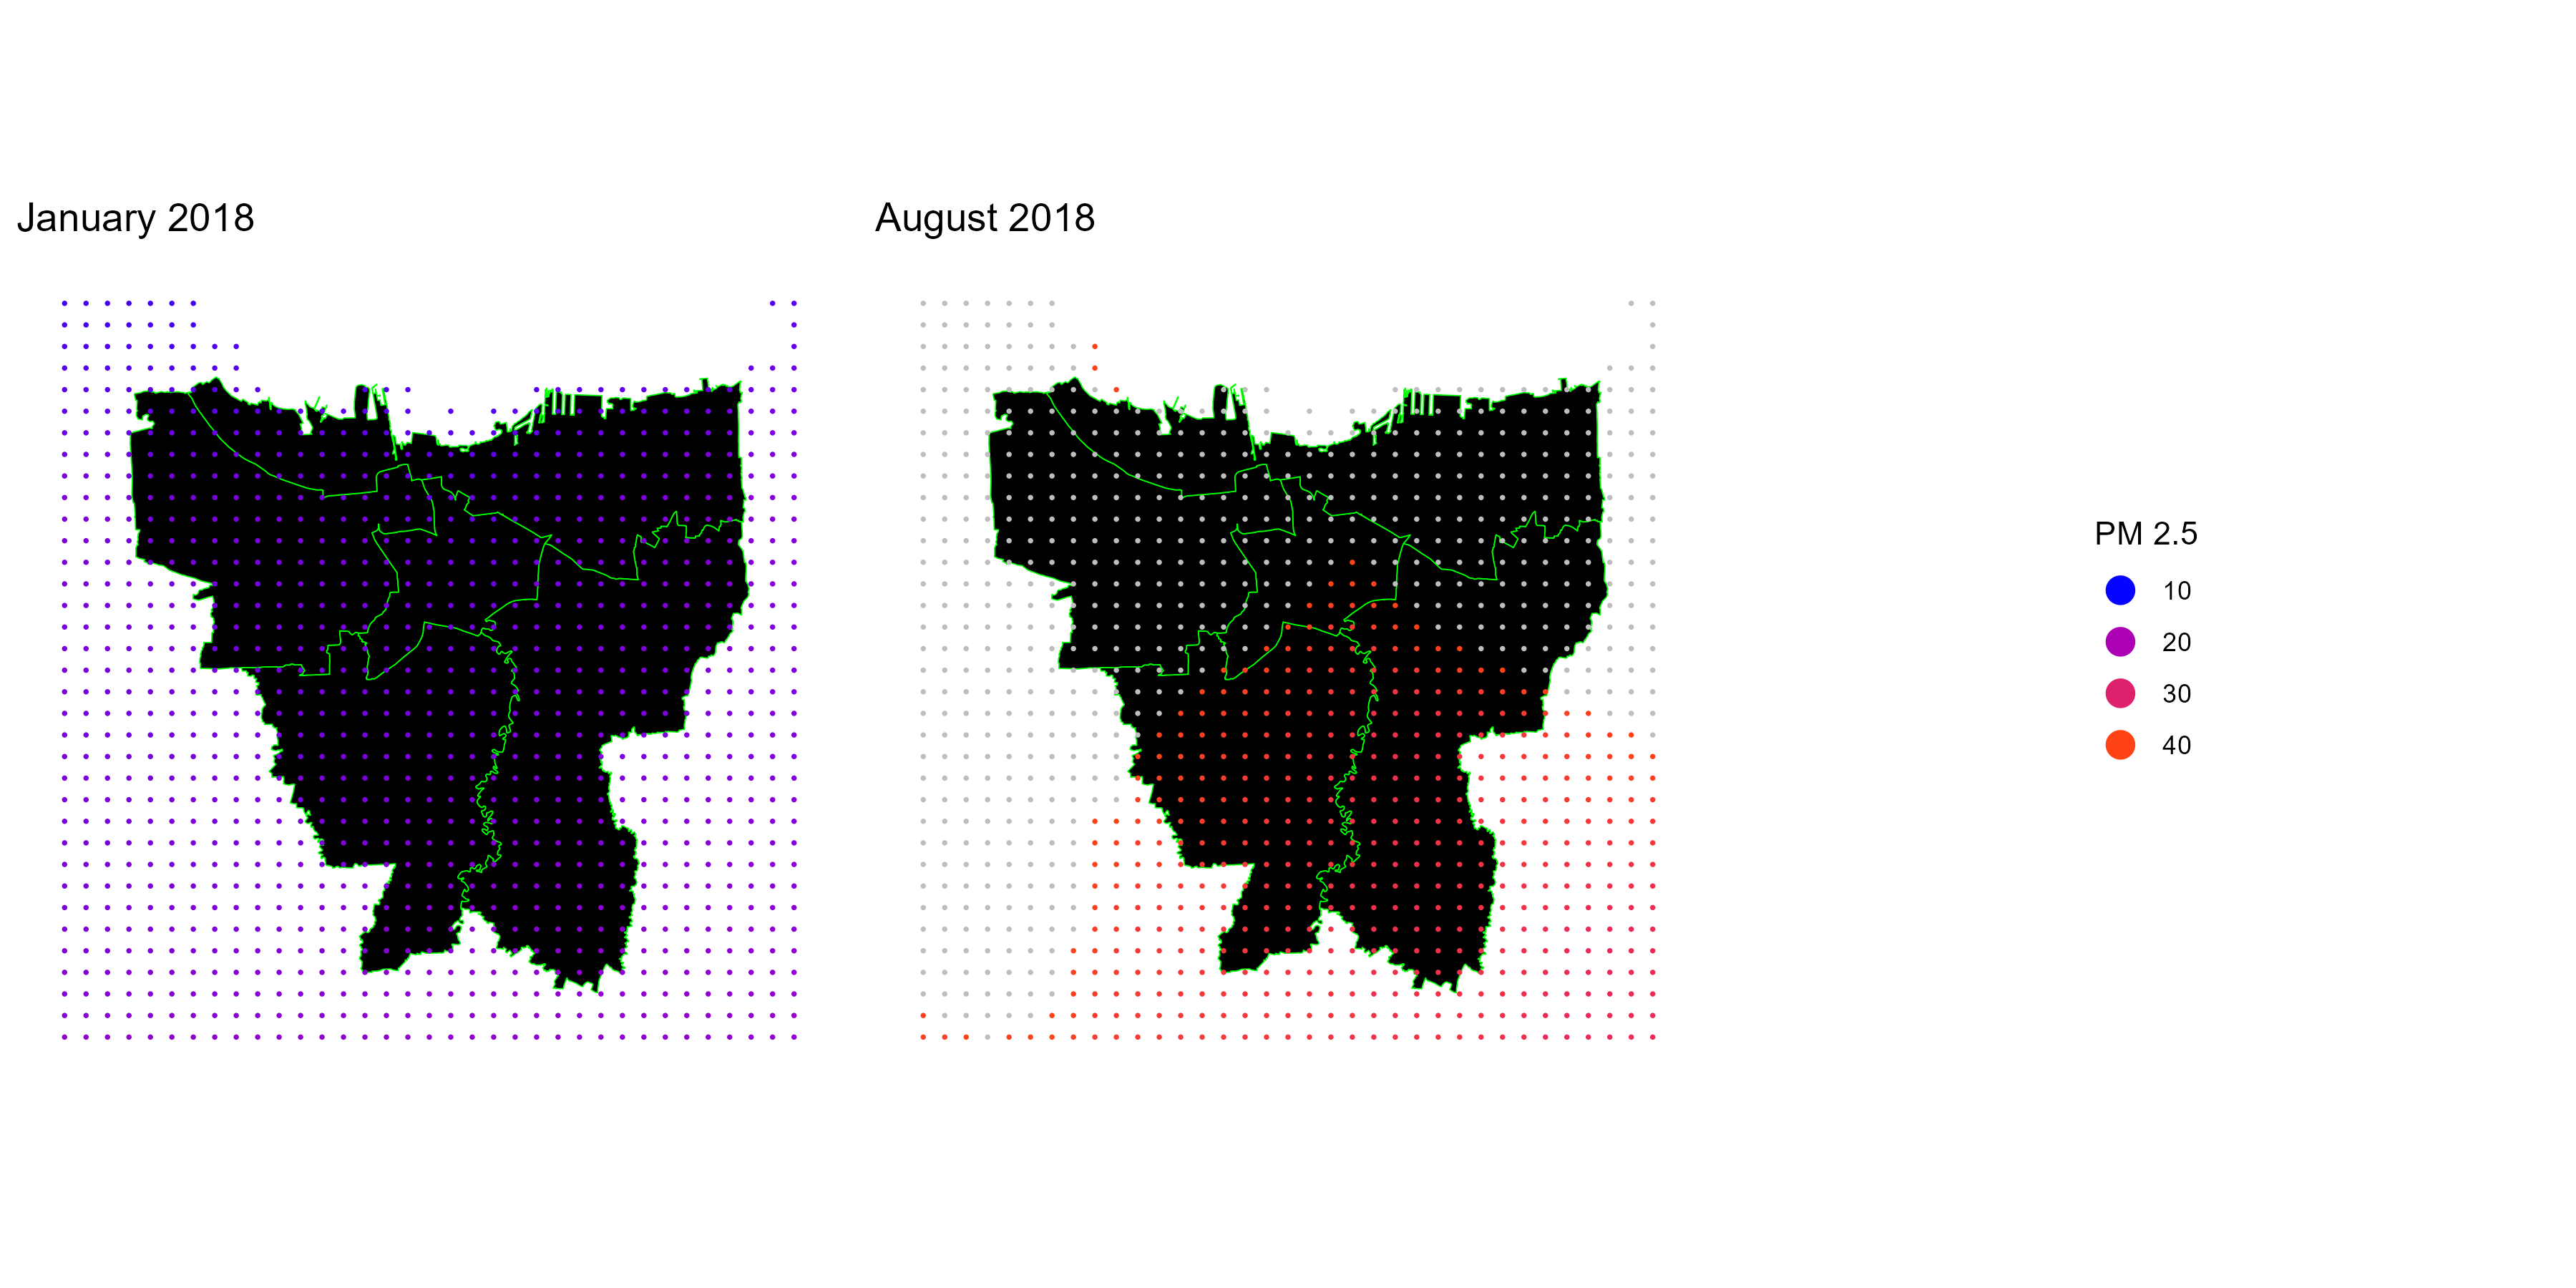
\includegraphics[width=1.2\linewidth]{Graphs/Jakarta_map.png}
    \vspace{-5em}
    \caption{Difference of PM2.5 on January and August 2018}
    \label{fig:Jakarta PM2.5 map on January and August 2018}
    \begin{figurenotes}
The PM2.5 is in $\mu$g$m^3$ unit. The blue area indicates the average of PM2.5 concentration is 10 $\mu$g$m^3$, while the red area indicates the average of PM2.5 was 40 $\mu$g$m^3$.
\end{figurenotes}
\begin{figurenotes}[Source]
Author's visualization using R.
\end{figurenotes}
\end{figure}
The Particulate Matter (PM) 2.5 data was obtained from the Van Donkelaar monthly average of global particulate matter (2021). This data is generated using satellite observation, which has been calibrated using actual ground-level measurements and modeled to fill if there is any gap. The observation unit of this data is a coordinate grid with a size of 0.01 x 0.01 degree, which roughly equals 1.1 x 1.1 km in the Jakarta region. Ideally, there are 1,113 satellite coordinate observations every month across the Jakarta region; however, in some cases, when the cloud is thick enough to prevent the satellite from measuring, the data will be null. Example of monthly data are presented below.



\vspace{15em}
\subsection{Roads}

The road data were obtained from the Open Street Map. The road data were then analyzed using the ArcGIS app to assign a dummy value to signify which road implements the odd-even policy, which would be our treatment road. The control roads were assigned to identify other roads with similar traffic loads as the comparison. This research uses primary roads that contain bus rapid transportation (BRT) system routes as the control roads because these roads should have similar characteristics as the treatment roads.

There are 9 road groups that implement the odd-even policy (\textit{1\_hayam\_wuruk} to \textit{9\_salemba}), while there is one group of roads that do not implement the odd-even policy as the control (\textit{0\_not\_gage}). The location of each road can be seen in the Background chapter.


\subsection{Rainfall}

Rainfall was obtained from Badan Pusat Statistik (BPS) or the National Statistical Bureau of Indonesia. This data is the result of observation at Kemayoran weather station. Rain can influence how long particulate matter can float in the air. Increasing rainfall should be correlated to lower particulate matter levels. As shown in Figure 3 below (red line), rainfall has an annual seasonality characteristic, which tends to be high earlier in the year (January - March) during the rainy season in Jakarta.

\begin{figure}
    \centering
    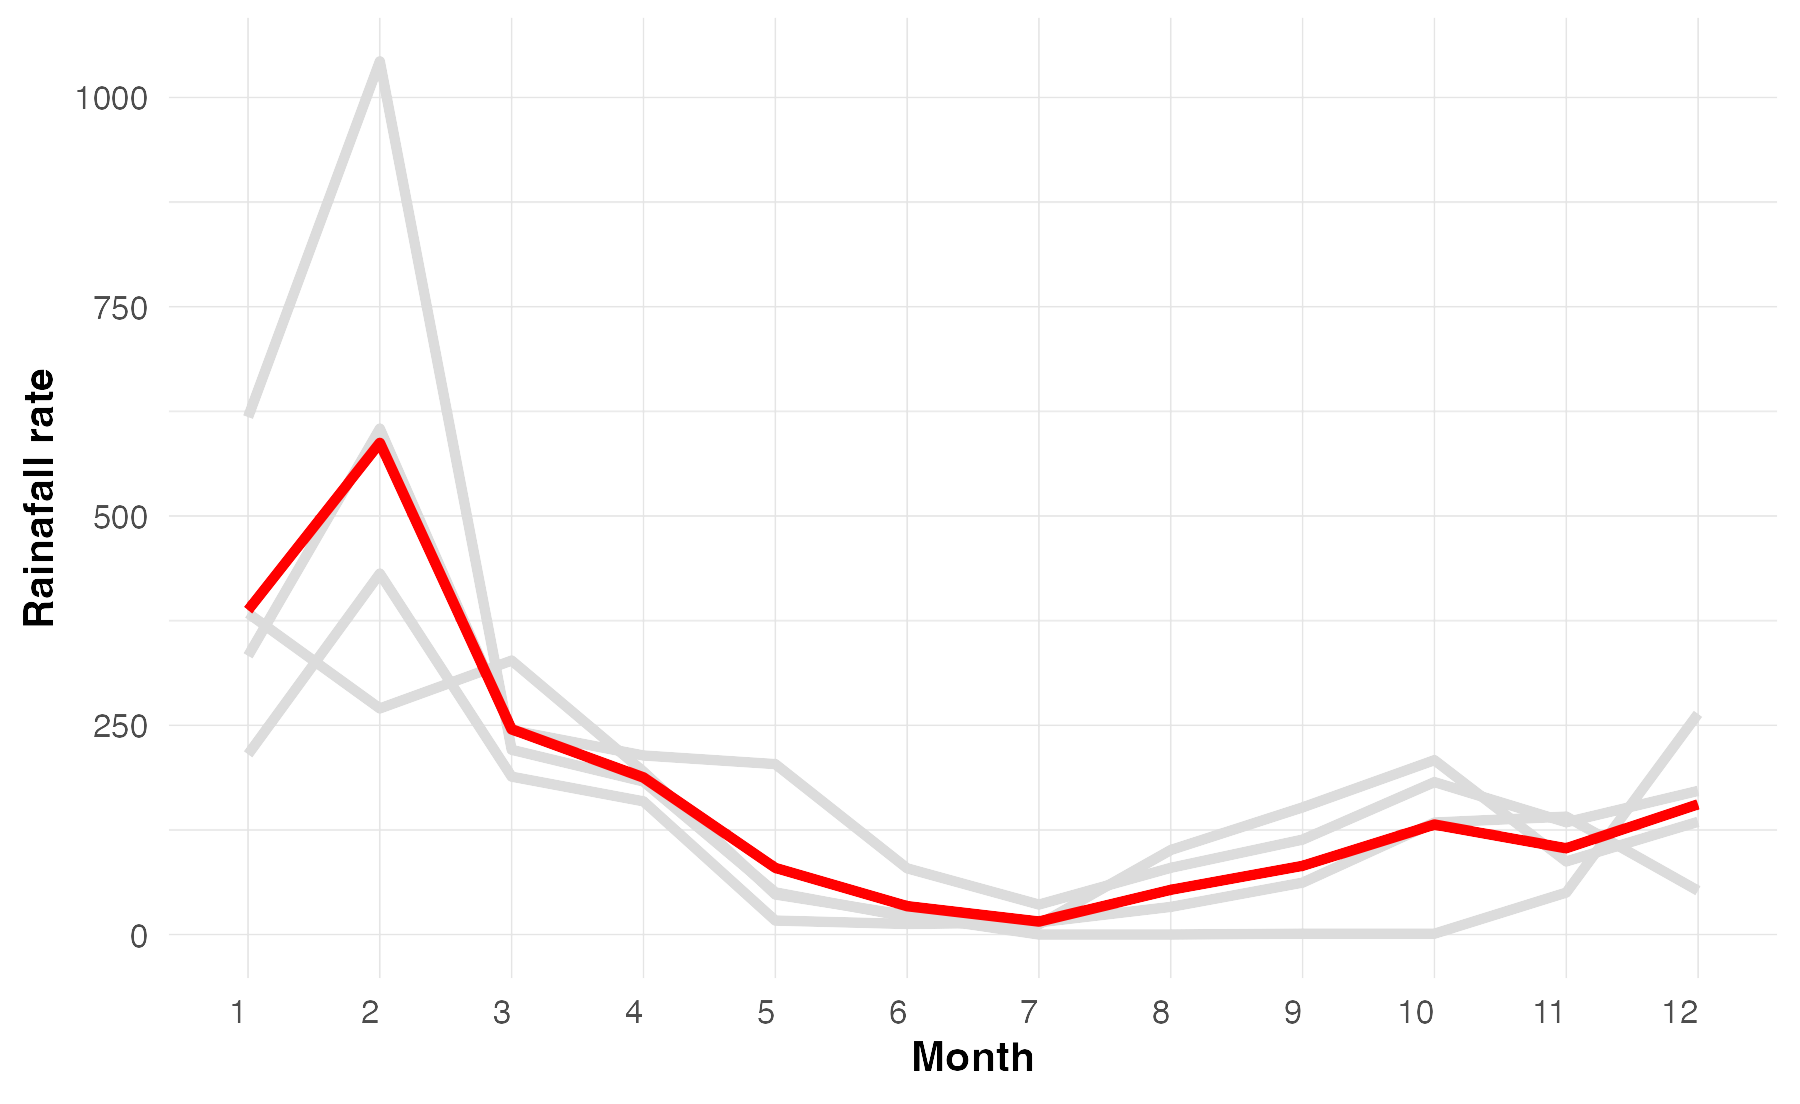
\includegraphics[width=0.8\linewidth]{Graphs/rain_seasonality_graph.png}
    \caption{Average Monthly Rainfall from 2018 to 2021 in Jakarta}
    \label{Average Monthly Rainfall from 2018 to 2021 in Jakarta}
    
\begin{figurenotes}[Source]
Author's visualization using R.
\end{figurenotes}
\end{figure}


\subsection{Holiday date}

Holiday date data was obtained from various sources, such as the Indonesian Cabinet Secretary's office website. This data shows various national holidays that impacted Jakarta's odd-even policy. There is one particular holiday that affects Jakarta's traffic condition, which is the Eid Al-Fitr holiday because this holiday is particularly lengthy, and Jakarta's population will go "mudik" or go to their hometown, which is usually located in the smaller cities throughout Indonesia. Therefore, Eid Al-Fitr holiday, instead of increasing traffic in Jakarta, this holiday would reduce traffic significantly.

\section{Exploratory Data Analysis}
\subsection{Seasonality Effect on Pollution} 

In addition to rainfall, as discussed in the previous chapter, particulate matter is also influenced by other weather events, such as wind and humidity. However, the month-fix effect is used instead due to the limitation of usable data. This approach should still be acceptable since most of the weather characteristic period is annual. This assumption is proven by statistically significant regression of the month as a dummy variable (and rainfall) with robust standard error. The seasonality can also be identified in Figure 4.

\begin{figure}
    \centering
    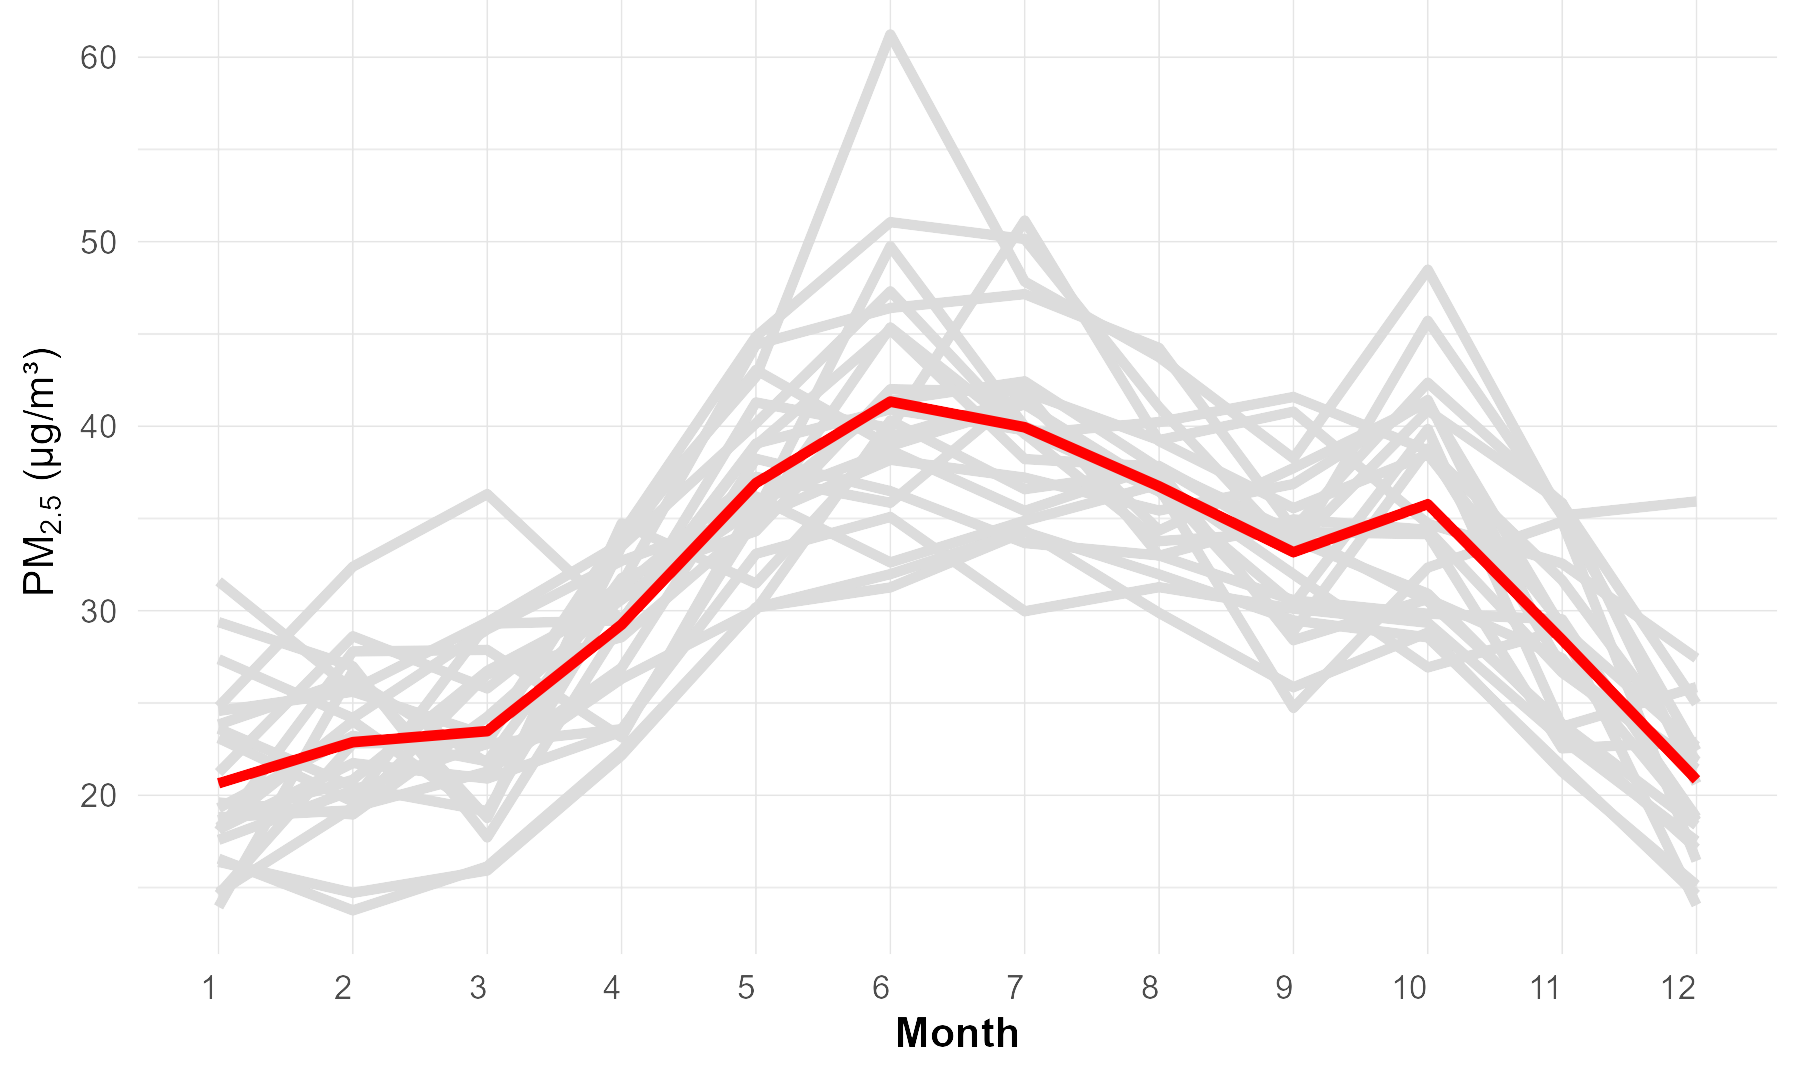
\includegraphics[width=0.8\linewidth]{Graphs/EDA_seasonality.png}
    \caption{Monthly Average of PM2.5 Concentration}
    \label{Seasonal PM2.5}
    \begin{figurenotes}[Source]
Author's visualization using R.
\end{figurenotes}
\end{figure}

Seasonality throughout the year has been also shown in the regression analysis in Table 1. For the whole months and years, the seasonal effects to PM2.5 pollution are statistically significant. In other words, seasons might induce bias that affects the concentration of PM2.5 and threaten the internal validity of the results. Therefore, there needs an empirical strategy to minimize the bias and strengthen the validity of the paper.

{\small
\begin{longtable}[]{@{}lrrr@{}}
\caption{Regression Results of Controlling Seasonality and
Holidays}\tabularnewline
\toprule\noalign{}
& (1) & (2) & (3) \\
\midrule\noalign{}
\endfirsthead
\toprule\noalign{}
& (1) & (2) & (3) \\
\midrule\noalign{}
\endhead
\bottomrule\noalign{}
\endlastfoot
(Intercept) & 0.102*** & 0.148*** & 0.277*** \\
& (0.102) & (0.148) & (0.277) \\
month2 & 0.145*** & 0.210*** & 0.219*** \\
& (0.145) & (0.210) & (0.219) \\
month3 & 0.145*** & 0.210*** & 0.225*** \\
& (0.145) & (0.210) & (0.225) \\
month4 & 0.162*** & 0.210*** & 0.229*** \\
& (0.162) & (0.210) & (0.229) \\
month5 & 0.162*** & 0.210*** & 0.304*** \\
& (0.162) & (0.210) & (0.304) \\
month6 & 0.162*** & 0.210*** & 0.307*** \\
& (0.162) & (0.210) & (0.307) \\
month7 & 0.162*** & 0.210*** & 0.306*** \\
& (0.162) & (0.210) & (0.306) \\
month8 & 0.162*** & 0.210*** & 0.294*** \\
& (0.162) & (0.210) & (0.294) \\
month9 & 0.162*** & 0.210*** & 0.278*** \\
& (0.162) & (0.210) & (0.278) \\
month10 & 0.162*** & 0.210*** & 0.240*** \\
& (0.162) & (0.210) & (0.240) \\
month11 & 0.162*** & 0.210*** & 0.237*** \\
& (0.162) & (0.210) & (0.237) \\
month12 & 0.162*** & 0.210*** & 0.283*** \\
& (0.162) & (0.210) & (0.283) \\
year2019 & & 0.210*** & 0.205*** \\
& & (0.210) & (0.205) \\
year2020 & & 0.210*** & 0.228*** \\
& & (0.210) & (0.228) \\
month2 × year2019 & & 0.296*** & 0.344*** \\
& & (0.296) & (0.344) \\
month3 × year2019 & & 0.296*** & 0.285*** \\
& & (0.296) & (0.285) \\
month4 × year2019 & & 0.296*** & 0.289*** \\
& & (0.296) & (0.289) \\
month5 × year2019 & & 0.296*** & 0.289*** \\
& & (0.296) & (0.289) \\
month6 × year2019 & & 0.296 & 0.292*** \\
& & (0.296) & (0.292) \\
month7 × year2019 & & 0.296*** & 0.296*** \\
& & (0.296) & (0.296) \\
month8 × year2019 & & 0.296*** & 0.300*** \\
& & (0.296) & (0.300) \\
month9 × year2019 & & 0.296*** & 0.307** \\
& & (0.296) & (0.307) \\
month10 × year2019 & & 0.296*** & 0.332*** \\
& & (0.296) & (0.332) \\
month11 × year2019 & & 0.296*** & 0.316*** \\
& & (0.296) & (0.316) \\
month12 × year2019 & & 0.296*** & 0.307*** \\
& & (0.296) & (0.307) \\
month2 × year2020 & & 0.296*** & 0.407*** \\
& & (0.296) & (0.407) \\
month3 × year2020 & & 0.296*** & \\
& & (0.296) & \\
rainfall & & & 0.001*** \\
& & & (0.001) \\
Num.Obs. & 30051 & 30051 & 30051 \\
R2 & 0.763 & 0.835 & 0.835 \\
R2 Adj. & 0.763 & 0.835 & 0.835 \\
AIC & 192139.1 & 181356.1 & 181356.1 \\
BIC & 192247.1 & 181588.8 & 181588.8 \\
Log.Lik. & -96056.545 & -90650.029 & -90650.029 \\
F & 8799.842 & & \\
RMSE & 5.92 & 4.94 & 4.94 \\
\end{longtable}

\textbf{Note:} \^{}\^{} + p \textless{} 0.1, * p \textless{} 0.05, ** p
\textless{} 0.01, *** p \textless{} 0.001

\textbf{Note:} \^{}\^{} Robust standard errors are used}

\subsection{Near Analysis}

This research's main interest is to evaluate road-level policy implementation. However, since the pollution data uses a coordinate observation unit, each grid is assigned to the nearest road. This
assignment was done through near-analysis geoprocessing in the ArcGIS software. This analysis resulted in the nearest distance from all observation coordinates to the selected roads.

Each observation coordinate is assigned to the nearest road and should be less than 1,000 meters from it. This analysis can also be imagined as
identifying coordinates within a 1,000 m buffer area from the roads. If the distance from the nearest road is more than 1,000 m, there will be no road assignment and will be given a null value.
The distribution of road-to-grid assignments is unequal, as shown in the table below. From 1,113 observations, 888 coordinates are located more than 1,000 meters from any roads of interest.


\begin{table}

\caption{\label{tab:unnamed-chunk-9}Distribution of Coordinates to the Nearest Roads}
\centering
\small\addtolength{\tabcolsep}{-4pt}
\begin{tabular}[t]{lr}
\toprule
Nearest Road & N\\
\midrule
0\_not\_gage & 162\\
1\_gajah\_mada & 3\\
2\_sudirman & 9\\
3\_fatmawati & 11\\
4\_tomang & 2\\
\addlinespace
5\_gatsu\_haryono & 16\\
6\_rasuna\_said & 3\\
7\_ahmad\_yani & 10\\
8\_pramuka & 3\\
9\_salemba & 6\\
\addlinespace
NA & 888\\
\bottomrule
\end{tabular}
\end{table}

\vspace{-1em}

\section{Empirical Strategy}

The odd-even policy motivates a straightforward fixed effect strategy
that estimates the causal effect of the policy and street pollution, comparing average levels of air pollution across months-year. The estimation equation is

\[
\small Y_{pm} = \beta_{1} S_{st}  + \mu_{s} + \tau_t + \varepsilon_{st}
\]

where \(\small Y_{pm}\) is the outcome of interest or the level of PM2.5 in raster observed by road \(\_{s}\) and time \(\_t\);
\(\small S\_{st}\) is a binary variable indicating treatment status (the odd-even policy), the road that implemented the policy becomes the
treatment group, while the control group is the street that never implements the policy but still has the same level of characteristics. The
coefficient of interest is \(\beta\_{1}\), which represents the average treatment effect between streets imposed with the odd-even policy and
not. \(\mu\_s\) represents street fixed effects that control for time-invariant shocks common to all streets; \(\tau\*t\*\) represents months-year fixed effects that control for time-varying shocks common to all streets, and \(\varepsilon{st}\) is an idiosyncratic error term.

These estimates may still have a bias from the difference in time when the policy was imposed because some roads implemented the policy in
August 2018, and the rest implemented the policy in September 2019. This bias might threaten internal validity and affect the conclusion. The event study research design can minimize this threat because it
estimates month-by-month effects relative to a base period (Goodman-Bacon, 2018). For the next step, this study incorporates event study into the estimation equation below.

\[
\tiny Y_{st} = 1\{\text{Odd-Even}\}[\sum_{y=-6}^{-2}\beta_{\text{pre}}\{t - t_s = y\} + \sum_{y=0}^{6}\beta_{\text{post}}\{t - t_s = y\}] + \mu_s + \tau_t + \varepsilon_{st}
\]

In the event study design, 1\{Odd Even Policy\} is a binary variable
identifying if a street is applied the odd-even policy, and \(t_s\) is
the month the policy was implemented. The coefficients of interest are
now \(\beta_{pre}\) and \(\beta_{post}\), which measure the effect
between the PM2.5 level and the odd-even policy in each of the 6 months
leading up to the policy and 6 months after.


\subsection{Difference in the Control and Treatment
Group}
Residuals are used for this analysis to control the seasonality effect based on previous analysis. Intuitively, this panel data shows that roads subject to the odd-even policy in most of the observed months have higher unexplained pollution (residuals). The differences between the two groups in Figure 5 below are not very clear. The regression table proves that even though the treatment group has higher unexplained pollution, the difference decreases after implementing the policy. This might indicate that the policy is successful in decreasing the pollution in the observed grid. However, since the implementation of the policy happened at two different times, an event study approach needs to be implemented. Two dashed lines represent two periods when the policy was implemented. Once in June 2018 and the other in September 2019.

\begin{figure}[hbt!]
    \centering
    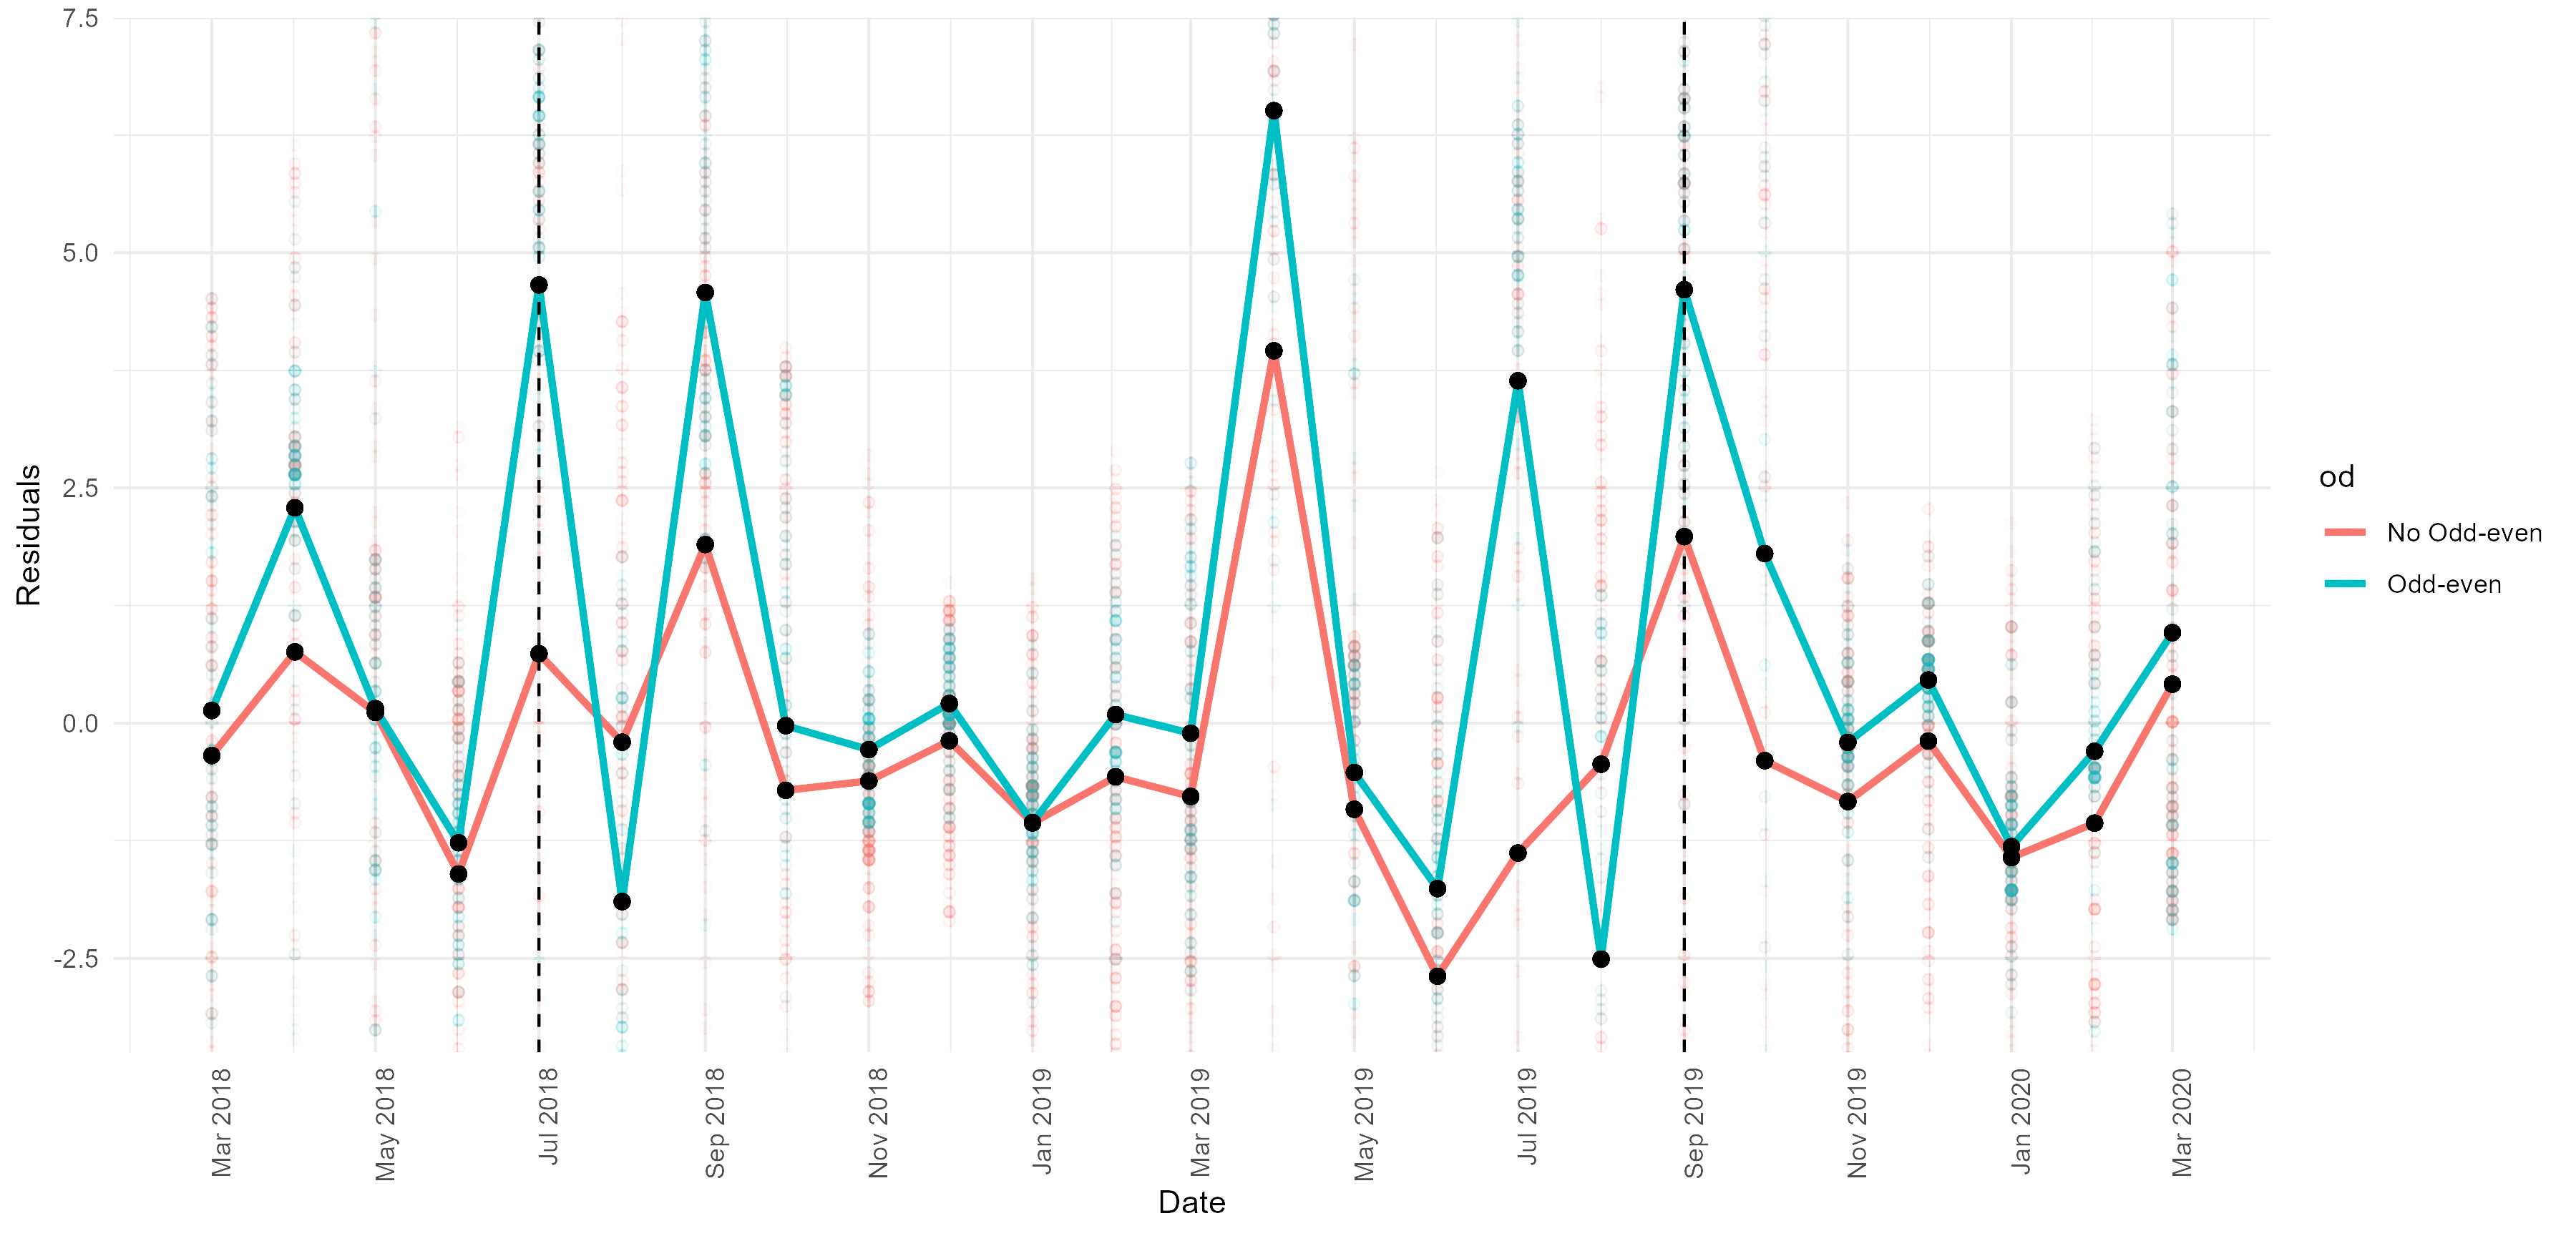
\includegraphics[width=1\linewidth]{Graphs/Graphoutput_plot.png}
    \caption{Average Residuals of Pollution Plot Over Time between Treatment and Control Groups}
    \label{fig:enter-label}
        \begin{figurenotes}[Source]
Author's visualization using R.
\end{figurenotes}
\end{figure}

{\small
\begin{longtable}[]{@{}lrr@{}}
\caption{Control and Treatment Difference Before and After
Policy}\tabularnewline
\toprule\noalign{}
& (1) & (2) \\
\midrule\noalign{}
\endfirsthead
\toprule\noalign{}
& (1) & (2) \\
\midrule\noalign{}
\endhead
\bottomrule\noalign{}
\endlastfoot
gage1 & 0.274*** & 0.207*** \\
& (0.274) & (0.207) \\
Num.Obs. & 1125 & 1575 \\
R2 & 0.012 & 0.015 \\
R2 Adj. & 0.011 & 0.015 \\
AIC & 6888.8 & 8725.8 \\
BIC & 6903.9 & 8741.9 \\
Log.Lik. & -3441.419 & -4359.885 \\
RMSE & 5.16 & 3.85 \\
Std.Errors & Custom & Custom \\
Before Policy & Yes & No \\
After Policy & No & Yes \\
\end{longtable}

\textbf{Note:} \^{}\^{} + p \textless{} 0.1, * p \textless{} 0.05, ** p
\textless{} 0.01, *** p \textless{} 0.001

\textbf{Note:} \^{}\^{} Robust standard errors are used}


\subsection{Event Study - Two Way Fixed
Effect}

Before the event study approach, this study estimates the effect of the
odd-even policy in the table column (1). The coefficient shows that the
policy reduces the PM2.5 by 1.5 $\mu$g$m^3$, on average, compared to
the road that did not implement the policy. After the event study, the coefficient in column (2) got larger compared to the
previous estimate. This shows average PM2.5 decreases by 1.9
$\mu$g$m^3$ in the Odd-even road. This is because the event study
minimizes the effect of unexpected factors between the first
implementation of the policy in August 2018 and September 2019 that
might reduce its magnitude. Finally, rainfall is
incorporated because this variable should have a high correlation with
PM2.5. However, column (3) shows that rainfall does not have a high
impact on pollution, and it is indicated by the coefficient of OD that
does not change.

The result of the two-way fixed effect using an event study is shown in the
chart below. The plot shows that the average PM2.5 decreased on the road
where the policy was implemented. However, a month later, the pollution
returned to the trend before the policy. Even though the coefficient of
\textit{Odd-even} from the table above indicates that the average pollution was
reduced due to the policy, the behavior of monthly pollution bounced
back a month after the policy.

\begin{figure}[hbt!]
    \centering
    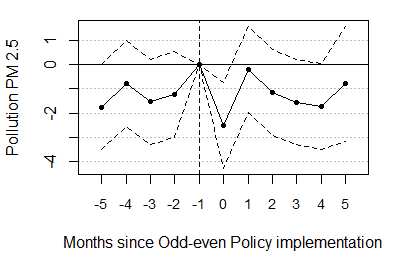
\includegraphics[width=0.6\linewidth]{Graphs/Rplot.png}
    \caption{To-way Fixed Effect Plot}
    \label{fig:enter-label}
        \begin{figurenotes}[Source]
Author's visualization using R.
\end{figurenotes}
\end{figure}

The plot of pollution residuals below also aligns with the findings of
``bounce back.'' This panel data shows that the unexplained pollution
(residuals) on the treated road was reduced after implementing the policy. This behavior was followed by the bounce back a month after the policy.


\begin{figure}[hbt!]
    \centering
    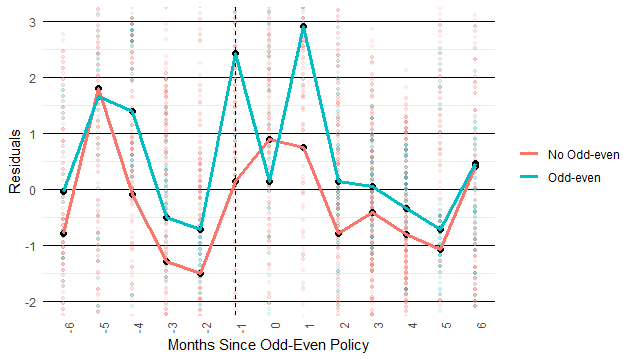
\includegraphics[width=0.8\linewidth]{Graphs/Rplot01.png}
    \caption{Average Residuals in Two-way Fixed Effect}
    \label{fig:enter-label}
            \begin{figurenotes}[Source]
Author's visualization using R.
\end{figurenotes}
\end{figure}

\section{Discussion}
\subsection{Policy Implication}
This research found that the odd-even policy is statistically
significant in terms of reducing air pollution, controlling the
month-year, rainfall, roads, and the event study. However, the 1.9
coefficient means that the policy does not reduce the PM 2.5 level to a
high degree, which means the pollution level reduction of the policy is
low. However, it is still an effective policy to reduce air pollution,
given the statistically significant result. This implies that if there
are no other policy alternatives to reduce air pollution in the region,
the expansion of this policy to other major or crowded roads should be
considered. Another reason for the odd-even policy expansion is the
significant result that the observed roads in the controlled roads, in
which there is no implementation of the policy, have higher PM 2.5
levels compared to the treatment roads. Assuming that the exposure to
pollution is the same between the control and treatment roads, the
implementation of the odd-even policy in the control roads would have
benefitted the population that lives nearby.

Another significant policy implication is the result of the event study.
The result of the event study shows that the most significant reduction
in PM 2.5 level was only in the first month after the policy was
implemented. While the overall trend after the policy implementation
still shows a pollution reduction, it is not as high as the reduction in
the first month. There are a few possibilities for why the reduction in
the first month is the largest one. First, it is regarding the
enforcement issues. As with any other regulation that passed in the
region, the initial implementation always met with tight enforcement.
This yields the pollution reduction that is expected by the policy.
However, after some time, it is often that the enforcement becomes much
more loose. This is also the possible explanation for the case in New
Delhi, where the University of Chicago research team measured the PM 2.5
level for the odd-even policy, and found that during the first month of
the implementation it decreased by 14\%-16\%, but no significant
reduction in the reinstatement. Another possibility is that the people
adapted to the policy, either by switching to a motorcycle, as it is not
regulated by the odd-even policy, or by buying another car with a
different plate number. The latter, for one, could be explained in
further research as this study does not observe the actual number of
cars on the road with the odd-even policy implementation.~

The government also needs take into consideration the cost of the policy,
as the odd-even restrictions on some roads limit the mobility of the
people, which, given that little transportation option is available,
could potentially harm the economic activities of the city. While the
debacle between the cost of limiting mobility and traffic congestion
remains, the implication of the policy is clear. The higher PM 2.5
levels in control roads, which are parallel to the BRT route, signify
that the effect of public transport provision on the air quality is
still low. Expansion of the public transportation system is needed to
compensate for the limitation of mobility, should the government decide
to expand the odd-even policy to other major roads.~

It should also be noted that there are no differences between the PM 2.5
level of the observation, whether the distance to the road is near or far
within the distance of 1000m. This means that the travel speed of PM 2.5
is high therefore the benefit of the odd-even policy should be a
citywide benefit instead of only benefitting the people who live near
the road that implements the policy.


\section{Conclusion}

This study reinforces the argument that restrictions on vehicle
operations have demonstrated a reduction of pollutant emissions (Bigazzi
and Rouleau, 2017). The odd-even policy in DKI Jakarta did manage to
reduce the PM 2.5 level, albeit only on a small scale. The results are also
consistent with the New Delhi case, which shows strongest effect in its
first month of implementation. It reflects the issues of enforcement of
the implementation, also the possibility of adaptation to the regulation
by the road users that reduce the efficacy of the policy, such as by
switching to motorcycles or buying another car with a different plate
number. Finally, the policy should be expanded, considering
limited alternatives to reduce air pollution in DKI Jakarta.


\newpage
\appendix

\section{Reference}

Bigazzi, A., Rouleau, M. (2017).~ Can traffic management strategies
improve urban air quality? A review of the evidence. Journal of
Transport \& Health, p.~111-124,
\url{https://doi.org/10.1016/j.jth.2017.08.001}.

Goodman-Bacon, A., (2018). ``Public Insurance and Mortality: Evidence
from Medicaid Implementation,'' Journal of Political Economy, University
of Chicago Press, vol.~126(1), pages 216-262. DOI: 10.1086/695528

Syuhada G, Akbar A, Hardiawan D, Pun V, Darmawan A, Heryati SHA, Siregar
AYM, Kusuma RR, Driejana R, Ingole V, Kass D, Mehta S. (2023).~ Impacts
of Air Pollution on Health and Cost of Illness in Jakarta, Indonesia.
Int J Environ Res Public Health. Feb 7;20(4):2916. doi:
10.3390/ijerph20042916.~

Zulkarnain, A.G., (2021). Impact of odd-even driving restrictions on air
quality in Jakarta. International Journal of Technology. Volume 12(5),
pp.~925-934

Is Delhi's odd-even scheme to battle air pollution even effective?
(2023). Energy Policy Institute at the University of Chicago.
\url{https://epic.uchicago.edu/news/is-delhis-odd-even-scheme-to-battle-air-pollution-even-effective/}

What you need to know about Jakarta's odd-even traffic policy. (2023).
The Jakarta Post.
\url{https://www.thejakartapost.com/news/2018/04/23/what-you-need-to-know-about-jakartas-odd-even-traffic-policy.html}


\end{document}

